% =====================================================================
%  tikzfigs.tex -- the small state machines, drawn instead of scanned.
%
%  \input by slides.tex.  These replace fig/ex1_coin.png,
%  fig/ex2_z1r.png, fig/ex3_rrxor.png, fig/ex4.png,
%  fig/ex4_redundant.png, fig/minimality.png and
%  fig/notation.png -- the diagrams in the deck that are just small
%  labelled digraphs.  Every state and edge below was read off the
%  transition matrices typeset beside it on the same slide, so the two
%  now cannot drift apart.
%
%  The larger hand-drawn conceptual figures (hierarchy, scope, pareto,
%  cave, instrumental, intervention, ...) deliberately stay as PNGs:
%  their freehand look is doing work that TikZ would flatten.
%
%  Colour follows the deck's own convention, the one already used in the
%  matrices: the emitted symbol is red, its probability blue.  \figNotation
%  stays black, because x and p there are variables, not particular values.
% =====================================================================

\usepackage{tikz}
\usetikzlibrary{arrows.meta, shapes.geometric, decorations.pathmorphing,
                backgrounds}

\tikzset{
  % a hidden state
  st/.style    = {draw, ellipse, inner sep=1pt, font=\small,
                  minimum width=9mm, minimum height=6.5mm},
  % an unlabelled state, for the minimality sketch
  blob/.style  = {draw, ellipse, minimum width=8mm, minimum height=5.5mm},
  % a transition
  tr/.style    = {-{Stealth[length=2.2mm,width=1.9mm]}, semithick},
  % an edge label
  el/.style    = {font=\scriptsize, inner sep=1.5pt},
  % the hand-drawn "reduces to" squiggle
  squig/.style = {-{Stealth[length=2.4mm,width=2.1mm]}, thick, gray,
                  decorate,
                  decoration={snake, amplitude=0.55mm, segment length=2.4mm,
                              post length=1.8mm}},
  % the highlight behind a redundant state
  hl/.style    = {fill=red!35, ellipse, minimum width=15mm, minimum height=11mm},
}

% emitted symbol : probability of emitting it
\newcommand{\eL}[2]{{\color{red}$#1$}\,{:}\,{\color{blue}$#2$}}

% ---------------------------------------------------------------------
%  Example 1 -- biased coin.  One state, T^(0) = 1-p, T^(1) = p.
% ---------------------------------------------------------------------
\newcommand{\figExOneCoin}{%
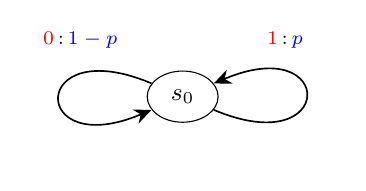
\begin{tikzpicture}
  \node[st] (s0) {$s_0$};
  \draw[tr] (s0) to[out=157,in=203,looseness=13] (s0);
  \draw[tr] (s0) to[out=-23,in=23,looseness=13]  (s0);
  \node[el] at (-1.30,0.72) {\eL{0}{1-p}};
  \node[el] at ( 1.30,0.72) {\eL{1}{p}};
\end{tikzpicture}}

% ---------------------------------------------------------------------
%  zero-one-random.  Example 2, and again as the reduction of Example 4.
%    T^(0): s0 -> s1 = 1,  sR -> s0 = 1-p
%    T^(1): s1 -> sR = 1,  sR -> s0 = p
%  #1 prefixes the node names, so the reduction can share one picture
%  with Example 4 without the two machines' s0/s1/sR colliding.
% ---------------------------------------------------------------------
\newcommand{\zorgraph}[1]{%
  \node[st] (#1s0) at (0,0)        {$s_0$};
  \node[st] (#1sR) at (3.3,0)      {$s_R$};
  \node[st] (#1s1) at (1.65,-1.85) {$s_1$};
  \draw[tr] (#1s0) -- node[el, below left]  {\eL{0}{1}}   (#1s1);
  \draw[tr] (#1s1) -- node[el, below right] {\eL{1}{1}}   (#1sR);
  \draw[tr] (#1sR) to[bend right=32] node[el, above] {\eL{1}{p}}   (#1s0);
  \draw[tr] (#1sR) to[bend left=15]  node[el, below] {\eL{0}{1-p}} (#1s0);
}

\newcommand{\figExTwoZOR}{%
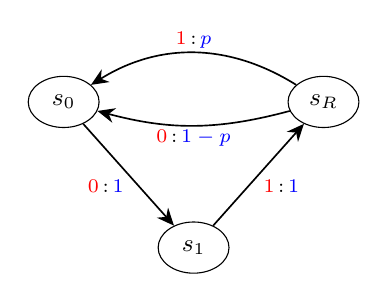
\begin{tikzpicture}\zorgraph{}\end{tikzpicture}}

% ---------------------------------------------------------------------
%  Example 3 -- random-random-XOR.
%    T^(0): so -> s0 = 1-p,  s0 -> sF = 1-q,  s1 -> sT = 1-q,  sF -> so = 1
%    T^(1): so -> s1 = p,    s0 -> sT = q,    s1 -> sF = q,    sT -> so = 1
% ---------------------------------------------------------------------
\newcommand{\figExThreeRRXOR}{%
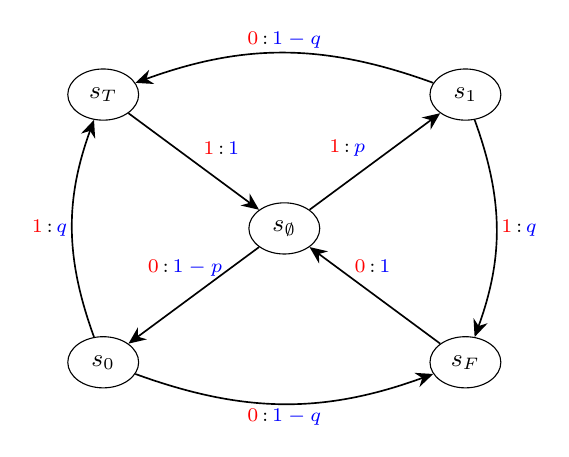
\begin{tikzpicture}
  \node[st] (sT) at (-2.3, 1.70) {$s_T$};
  \node[st] (s1) at ( 2.3, 1.70) {$s_1$};
  \node[st] (se) at ( 0.0, 0.00) {$s_\emptyset$};
  \node[st] (s0) at (-2.3,-1.70) {$s_0$};
  \node[st] (sF) at ( 2.3,-1.70) {$s_F$};
  % rim
  \draw[tr] (s1) to[bend right=20] node[el, above] {\eL{0}{1-q}} (sT);
  \draw[tr] (s1) to[bend left=20]  node[el, right] {\eL{1}{q}}   (sF);
  \draw[tr] (s0) to[bend left=20]  node[el, left]  {\eL{1}{q}}   (sT);
  \draw[tr] (s0) to[bend right=20] node[el, below] {\eL{0}{1-q}} (sF);
  % spokes
  \draw[tr] (sT) -- (se);
  \draw[tr] (se) -- (s1);
  \draw[tr] (se) -- (s0);
  \draw[tr] (sF) -- (se);
  \node[el] at (-0.80, 1.02) {\eL{1}{1}};
  \node[el] at ( 0.80, 1.02) {\eL{1}{p}};
  \node[el] at (-1.26,-0.50) {\eL{0}{1-p}};
  \node[el] at ( 1.12,-0.48) {\eL{0}{1}};
\end{tikzpicture}}

% ---------------------------------------------------------------------
%  Example 4.
%    T~^(0): s0 -> s1 = q,  s0 -> s2 = 1-q,  sR -> s0 = 1-p
%    T~^(1): s1 -> sR = 1,  s2 -> sR = 1,    sR -> s0 = p
% ---------------------------------------------------------------------
\newcommand{\exfourgraph}{%
  \node[st] (s2) at ( 0.00, 1.85) {$s_2$};
  \node[st] (s0) at (-2.05, 0.00) {$s_0$};
  \node[st] (sR) at ( 2.05, 0.00) {$s_R$};
  \node[st] (s1) at ( 0.00,-1.85) {$s_1$};
  \draw[tr] (s0) -- node[el, above left]  {\eL{0}{1-q}} (s2);
  \draw[tr] (s2) -- node[el, above right] {\eL{1}{1}}   (sR);
  \draw[tr] (s0) -- node[el, below left]  {\eL{0}{q}}   (s1);
  \draw[tr] (s1) -- node[el, below right] {\eL{1}{1}}   (sR);
  \draw[tr] (sR) to[bend right=22] node[el, above] {\eL{1}{p}}   (s0);
  \draw[tr] (sR) to[bend left=11]  node[el, below] {\eL{0}{1-p}} (s0);
}

\newcommand{\figExFour}{%
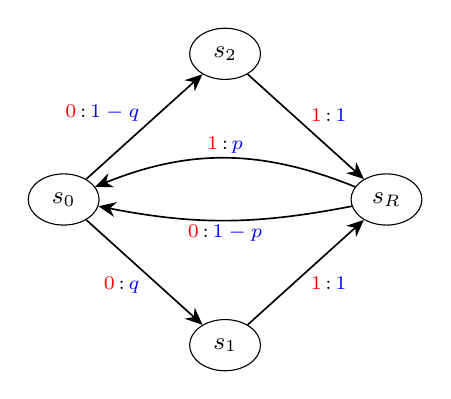
\begin{tikzpicture}\exfourgraph\end{tikzpicture}}

% ---------------------------------------------------------------------
%  Example 4 again, with s2 marked redundant and the machine reduced.
%  The reduction is exactly zero-one-random, hence \zorgraph here too.
% ---------------------------------------------------------------------
\newcommand{\figExFourRedundant}{%
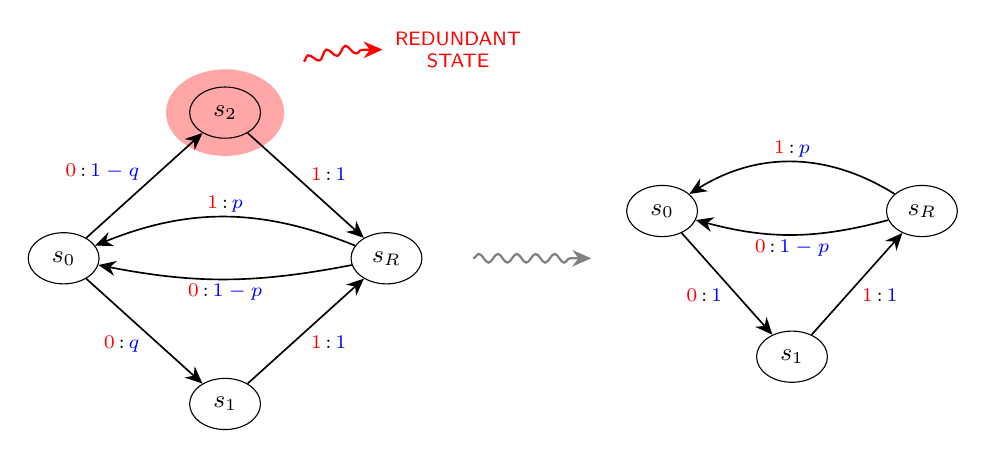
\begin{tikzpicture}
  \exfourgraph
  \begin{scope}[on background layer]
    \node[hl] at (s2) {};
  \end{scope}
  \draw[squig, red] (1.00,2.50) to[out=20,in=180] (2.00,2.65);
  \node[el, red, anchor=west, align=center, font=\scriptsize\sffamily]
        at (2.10,2.65) {REDUNDANT\\STATE};
  \draw[squig] (3.15,0) -- (4.65,0);
  \begin{scope}[shift={(5.55,0.60)}]
    \zorgraph{r}
  \end{scope}
\end{tikzpicture}}

% ---------------------------------------------------------------------
%  Notation.  x and p are variables here, so this one is not coloured.
% ---------------------------------------------------------------------
\newcommand{\figNotation}{%
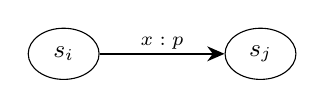
\begin{tikzpicture}[baseline=(si.base)]
  \node[st] (si) at (0,0)   {$s_i$};
  \node[st] (sj) at (2.5,0) {$s_j$};
  \draw[tr] (si) -- node[el, above] {$x : p$} (sj);
\end{tikzpicture}}

% ---------------------------------------------------------------------
%  Minimality -- the same process realised by ever fewer hidden states.
%  The states are deliberately unlabelled in the original: the point is
%  the shrinking state count, not any particular machine.
% ---------------------------------------------------------------------
\newcommand{\figMinimality}{%
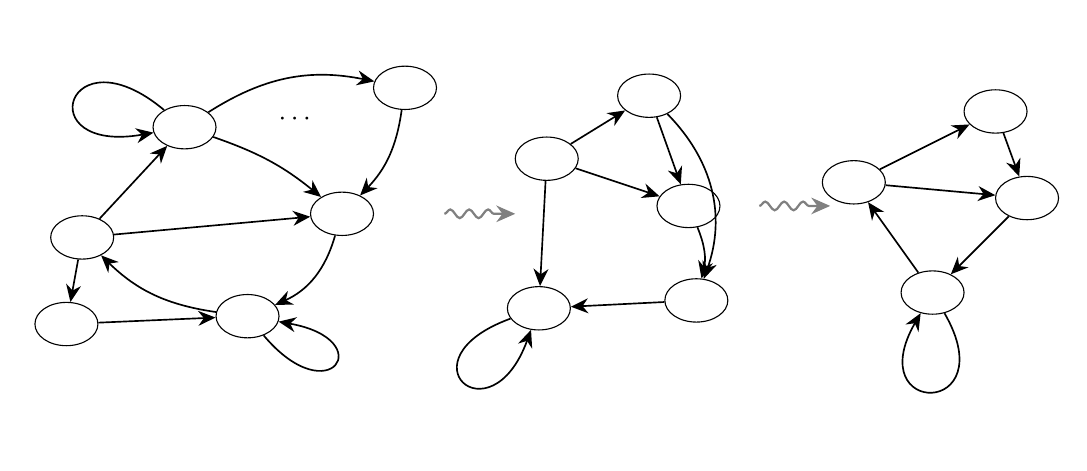
\begin{tikzpicture}[x=1mm, y=1mm]
  % --- six states, with more elided ---
  \begin{scope}
    \node[blob] (a1) at (15,25) {};
    \node[blob] (a2) at (43,30) {};
    \node[blob] (a3) at (35,14) {};
    \node[blob] (a4) at ( 2,11) {};
    \node[blob] (a5) at ( 0, 0) {};
    \node[blob] (a6) at (23, 1) {};
    \node       (ad) at (29,26) {$\cdots$};
    \draw[tr] (a1) to[out=140,in=190,looseness=13] (a1);
    \draw[tr] (a1) to[bend left=22]  (a2);
    \draw[tr] (a1) to[bend left=10]  (a3);
    \draw[tr] (a2) to[bend left=18]  (a3);
    \draw[tr] (a4) -- (a1);
    \draw[tr] (a4) -- (a3);
    \draw[tr] (a4) -- (a5);
    \draw[tr] (a3) to[bend left=25]  (a6);
    \draw[tr] (a5) -- (a6);
    \draw[tr] (a6) to[bend left=18]  (a4);
    \draw[tr] (a6) to[out=-50,in=-10,looseness=13] (a6);
  \end{scope}
  % --- five ---
  \begin{scope}[shift={(60,2)}]
    \node[blob] (b1) at (14,27) {};
    \node[blob] (b2) at ( 1,19) {};
    \node[blob] (b3) at (19,13) {};
    \node[blob] (b4) at ( 0, 0) {};
    \node[blob] (b5) at (20, 1) {};
    \draw[tr] (b2) -- (b1);
    \draw[tr] (b1) -- (b3);
    \draw[tr] (b1) to[bend left=32] (b5);
    \draw[tr] (b2) -- (b3);
    \draw[tr] (b2) -- (b4);
    \draw[tr] (b3) to[bend left=18] (b5);
    \draw[tr] (b5) -- (b4);
    \draw[tr] (b4) to[out=200,in=250,looseness=13] (b4);
  \end{scope}
  % --- four ---
  \begin{scope}[shift={(100,4)}]
    \node[blob] (c1) at (18,23) {};
    \node[blob] (c2) at ( 0,14) {};
    \node[blob] (c3) at (22,12) {};
    \node[blob] (c4) at (10, 0) {};
    \draw[tr] (c2) -- (c1);
    \draw[tr] (c1) -- (c3);
    \draw[tr] (c2) -- (c3);
    \draw[tr] (c3) -- (c4);
    \draw[tr] (c4) -- (c2);
    \draw[tr] (c4) to[out=-60,in=-120,looseness=13] (c4);
  \end{scope}
  % --- and the reductions between them ---
  \draw[squig] (48,14) -- (57,14);
  \draw[squig] (88,15) -- (97,15);
\end{tikzpicture}}
